\documentclass[a4paper]{article}
\usepackage{times}
\usepackage[utf8]{inputenc}
\usepackage{selinput}
\usepackage{upquote}
\usepackage[margin=2cm, rmargin=4cm, tmargin=3cm]{geometry}
\usepackage{tcolorbox}
\usepackage{xspace}
\usepackage[french]{babel}
\usepackage{url}
\usepackage{hyperref}
\usepackage{fontawesome5}
\usepackage{marginnote}
\usepackage{ulem}
\usepackage{tcolorbox}
\usepackage{graphicx}
%\usepackage[top=Bcm, bottom=Hcm, outer=Ccm, inner=Acm, heightrounded, marginparwidth=Ecm, marginparsep=Dcm]{geometry}


\newtcolorbox{Example}[1]{colback=white,left=20pt,colframe=slideblue,fonttitle=\bfseries,title=#1}
\newtcolorbox{Solutions}[1]{colback=white,left=20pt,colframe=green,fonttitle=\bfseries,title=#1}
\newtcolorbox{Conseils}[1]{colback=white,left=20pt,colframe=slideblue,fonttitle=\bfseries,title=#1}
\newtcolorbox{Warning}[1]{colback=white,left=20pt,colframe=warning,fonttitle=\bfseries,title=#1}

\setlength\parindent{0pt}

  %Exercice environment
  \newcounter{exercice}
  \newenvironment{Exercice}[1][]
  {
  \par
  \stepcounter{exercice}\textbf{Question \arabic{exercice}:} (\faClock \enskip \textit{#1})
  }
  {\bigskip}
  

% Title
\newcommand{\titre}{\begin{center}
  \section*{Algorithmes et Pensée Computationnelle}
\end{center}}
\newcommand{\cours}[1]
{\begin{center} 
  \textit{#1}\\
\end{center}
  }


\newcommand{\exemple}[1]{\newline~\textbf{Exemple :} #1}
%\newcommand{\attention}[1]{\newline\faExclamationTriangle~\textbf{Attention :} #1}

% Documentation url (escape \# in the TP document)
\newcommand{\documentation}[1]{\faBookOpen~Documentation : \href{#1}{#1}}

% Clef API
\newcommand{\apikey}[1]{\faKey~Clé API : \lstinline{#1}}
\newcommand{\apiendpoint}[1]{\faGlobe~Url de base de l'API \href{#1}{#1}}

%Listing Python style
\usepackage{color}
\definecolor{slideblue}{RGB}{33,131,189}
\definecolor{green}{RGB}{0,190,100}
\definecolor{blue}{RGB}{121,142,213}
\definecolor{grey}{RGB}{120,120,120}
\definecolor{warning}{RGB}{235,186,1}

\usepackage{listings}
\lstdefinelanguage{texte}{
    keywordstyle=\color{black},
    numbers=none,
    frame=none,
    literate=
           {é}{{\'e}}1
           {è}{{\`e}}1
           {ê}{{\^e}}1
           {à}{{\`a}}1
           {â}{{\^a}}1
           {ù}{{\`u}}1
           {ü}{{\"u}}1
           {î}{{\^i}}1
           {ï}{{\"i}}1
           {ë}{{\"e}}1
           {Ç}{{\,C}}1
           {ç}{{\,c}}1,
    columns=fullflexible,keepspaces,
	breaklines=true,
	breakatwhitespace=true,
}
\lstset{
    language=Python,
	basicstyle=\bfseries\footnotesize,
	breaklines=true,
	breakatwhitespace=true,
	commentstyle=\color{grey},
	stringstyle=\color{slideblue},
  keywordstyle=\color{slideblue},
	morekeywords={with, as, True, False, Float, join, None, main, argparse, self, sort, __eq__, __add__, __ne__, __radd__, __del__, __ge__, __gt__, split, os, endswith, is_file, scandir, @classmethod},
	deletekeywords={id},
	showspaces=false,
	showstringspaces=false,
	columns=fullflexible,keepspaces,
	literate=
           {é}{{\'e}}1
           {è}{{\`e}}1
           {ê}{{\^e}}1
           {à}{{\`a}}1
           {â}{{\^a}}1
           {ù}{{\`u}}1
           {ü}{{\"u}}1
           {î}{{\^i}}1
           {ï}{{\"i}}1
           {ë}{{\"e}}1
           {Ç}{{\,C}}1
           {ç}{{\,c}}1,
    numbers=left,
}

\newtcbox{\mybox}{nobeforeafter,colframe=white,colback=slideblue,boxrule=0.5pt,arc=1.5pt, boxsep=0pt,left=2pt,right=2pt,top=2pt,bottom=2pt,tcbox raise base}
\newcommand{\projet}{\mybox{\textcolor{white}{\small projet}}\xspace}
\newcommand{\optionnel}{\mybox{\textcolor{white}{\small Optionnel}}\xspace}
\newcommand{\advanced}{\mybox{\textcolor{white}{\small Pour aller plus loin}}\xspace}
\newcommand{\auto}{\mybox{\textcolor{white}{\small Auto-évaluation}}\xspace}


\usepackage{environ}
\newif\ifShowSolution
\NewEnviron{solution}{
  \ifShowSolution
	\begin{Solutions}{\faTerminal \enskip Solution}
		\BODY
	\end{Solutions}
  \fi}


  \usepackage{environ}
  \newif\ifShowConseil
  \NewEnviron{conseil}{
    \ifShowConseil
    \begin{Conseils}{\faLightbulb \quad Conseil}
      \BODY
    \end{Conseils}

    \fi}

    \usepackage{environ}
  \newif\ifShowWarning
  \NewEnviron{attention}{
    \ifShowWarning
    \begin{Warning}{\faExclamationTriangle \quad Attention}
      \BODY
    \end{Warning}

    \fi}
  

%\newcommand{\Conseil}[1]{\ifShowIndice\ \newline\faLightbulb[regular]~#1\fi}


\usepackage{array}
\newcolumntype{C}[1]{>{\centering\let\newline\\\arraybackslash\hspace{0pt}}m{#1}}

\begin{document}
% Change the following values to true to show the solutions or/and the hints
\ShowSolutiontrue
\ShowConseiltrue
\titre
\cours{Consolidation 1}

Les exercices de cette série sont une compilation d'exercices semblables à ceux vu lors des semaines précédentes. Le but de cette séance est de consolider les connaissances acquises lors des travaux pratiques des semaines 1 à 6.

Le code présenté dans les énoncés se trouve sur Moodle, dans le dossier \lstinline{Ressources}.


\section{Introduction et architecture des ordinateurs}

\subsection{Introduction/Résumé}

Le but de cette section est de comprendre le fonctionnement d'un ordinateur. La série d'exercices sera axée autour de conversions en base binaire, décimale, hexadécimale, base 5 et de calcul de base en suivant le modèle Von Neumann. \\

\subsection{Conversion}

\begin{Exercice}[10 minutes]  \textbf{Conversion }\\
    \begin{enumerate}
        \item Convertir le nombre FFFFFF$_{(16)}$ en base 10.
        \item Convertir le nombre 4321$_{(5)}$ en base 10.
        \item Convertir le nombre ABC$_{(16)}$ en base 2.
        \item Convertir le nombre 254$_{(10)}$ en base 15.
        \item Convertir le nombre 11101$_{(2)}$ en base 10.
    \end{enumerate}
    
        \begin{conseil}
            N'oubliez pas qu'en Hexadécimal, A vaut 10, B vaut 11, C vaut 12, D vaut 13, E vaut 14 et F vaut 15.
    \end{conseil}

    \begin{solution}
        1. FFFFFF$_{(16)}$ = 16777215$_{(10)}$\\
        2. 4321$_{(5)}$ = 586$_{(10)}$\\
        3. ABC$_{(16)}$ = 101010111100$_{(2)}$\\
        4. 254$_{(10)}$ = 11E$_{(15)}$\\
        5. 11101$_{(2)}$ = 29$_{(10)}$
    \end{solution}
\end{Exercice}

\begin{comment}
    % Les étudiants n'ont pas rencontré de difficultés sur des exercices similaires
\subsection{Arithmétique binaire}

\begin{Exercice}[5 minutes] \textbf{Addition et soustraction de nombres binaires}
    \begin{enumerate}
        \item Additionner \lstinline{10110101}$_{(2)}$ et \lstinline{00010101}$_{(2)}$
        \item Soustraire \lstinline{11000101}$_{(2)}$ et \lstinline{01000000}$_{(2)}$

    \end{enumerate}
    
     \begin{conseil}
        Cf: exercice 4,5 week 1
    \end{conseil}
    
  

    \begin{solution}
        1. {10110101}$_{(2)}$ + {00010101}$_{(2)}$ = {11001010}$_{(2)}$\\
        2. {11000101}$_{(2)}$ - {01000000}$_{(2)}$ = {10000101}$_{(2)}$
    \end{solution}
\end{Exercice}








\end{comment}
\subsection{Conversion et arithmétique}
\begin{Exercice}[5 minutes] \textbf{Conversion, addition et soustraction:}\\
    Effectuer les opérations suivantes:
    \begin{enumerate}
        \item 10110101$_{(2)}$ + 00101010$_{(2)}$ = ...$_{(10)}$
        \item 70$_{(10)}$ - 10101010$_{(2)}$ = ...$_{(10)}$
    \end{enumerate}
        \begin{conseil}
        Convertissez dans une base commune avant d'effectuer les opérations.
    \end{conseil}
        
    \begin{solution}
        1. 10110101$_{(2)}$ + 00101010$_{(2)}$ = 223$_{(10)}$\\
        3. 70$_{(10)}$ - 10101010$_{(2)}$ = -100$_{(10)}$
    \end{solution}
\end{Exercice}


\subsection{Modèle de Von Neuman}
Dans cette section, nous allons simuler une opération d'addition dans le \textbf{modèle de Van Neumann}, il va vous être demandé à chaque étape (FDES) de donner la valeur des registres.\\

\textbf{État d'origine:}\\
A l'origine, notre \lstinline{Process Counter (PC)} vaut \lstinline{00100001}.\\

Dans la mémoire, les instructions sont les suivantes:

\begin{tabular}{| C{0.1\textwidth} | C{0.1\textwidth} |} 
    \hline
    \textbf{Adresse} & \textbf{Valeur}\\ [0.5ex]
    \hline
    00100001 & 00110100\\ [0.5ex] 
    \hline
    00101100 & 10100110\\ [0.5ex] 
    \hline
    01110001 & 111111101\\ [0.5ex]
    \hline
\end{tabular}
\\\\
Les registres sont les suivants:

\begin{tabular}{| C{0.1\textwidth} | C{0.1\textwidth} |} 
    \hline
    \textbf{Registre} & \textbf{Valeur}\\ [0.5ex]
    \hline
    00 & 01111111\\ [0.5ex] 
    \hline
    01 & 00100000\\ [0.5ex] 
    \hline
    10 & 00101101\\ [0.5ex] 
    \hline
    11 & 00001100\\ [0.5ex]
    \hline
\end{tabular}
\\\\
Les opérations disponibles pour l'unité de contrôle sont les suivantes:
\\
\begin{tabular}{| C{0.1\textwidth} | C{0.1\textwidth} |} 
    \hline
    \textbf{Numéro} & \textbf{Valeur}\\ [0.5ex]
    \hline
    00 & ADD\\ [0.5ex] 
    \hline
    01 & XOR\\ [0.5ex] 
    \hline
    10 & MOV\\ [0.5ex] 
    \hline
    11 & SUB\\ [0.5ex]
    \hline
\end{tabular}
\\\\


\begin{Exercice}[5 minutes]\textbf{Fetch}\\
    À la fin de l'opération \lstinline{FETCH}, quelles sont les valeurs du \lstinline{Process Counter} et de l'\lstinline{Instruction Register}?
\end{Exercice}
   \begin{conseil}
    Pour rappel, l’unité de contrôle (Control Unit) commande et contrôle le fonctionnement du système. Elle est chargée du séquençage des opérations. Après chaque opération FETCH, la valeur du Program Counter est incrémentée (valeur initiale + 1).
    \end{conseil}
\begin{solution}
    PC = 00100001$_{(2)}$ + 1 = 00100010$_{(2)}$\\
    IR = 00110100$_{(2)}$
\end{solution}

\begin{Exercice}[5 minutes] \textbf{Decode}
    \begin{enumerate}
        \item Quelle est la valeur de l'opération à exécuter?
        \item Quelle est l'adresse du registre dans lequel le résultat doit être enregistré?
        \item Quelle est la valeur du premier nombre de l'opération?
        \item Quelle est la valeur du deuxième nombre de l'opération?
    \end{enumerate}
\end{Exercice}
   \begin{conseil}
    Pensez à décomposer la valeur de l’\lstinline{Instruction Register} pour obtenir toutes les informations demandées.\\
    Utilisez la même convention que celle présentée dans les diapositives du cours (Architecture des ordinateurs (Semaine 2) - Diapositive 15)\\
    Les données issues de la décomposition de l’\lstinline{Instruction Register} ne sont pas des valeurs brutes, mais des références. Trouvez les tables concordantes pour y récupérer les valeurs.

    \end{conseil}
\begin{solution}
    00 : \lstinline{ADD} (valeur de l'opération à exécuter)\\
    11 : Adresse du registre dans lequel le résultat doit être enregistré\\
    01 : 00100000$_{(2)}$ (premier nombre)\\
    00 : 01111111$_{(2)}$ (deuxième nombre)
\end{solution}

\begin{Exercice}[5 minutes] \textbf{Execute}\\
    Quel est résultat de l'opération?
\end{Exercice}

   \begin{conseil}
        Toutes les informations permettant d’effectuer l’opération se trouvent dans les données de l’\lstinline{Instruction Register}.
    \end{conseil}

\begin{solution}
    00100000$_{(2)}$ + 01111111$_{(2)}$ = 10011111$_{(2)}$
\end{solution}


% Week 2
\section{Logiciels système}

\subsection{Introduction/Résumé}

\subsection{Operating system}

\begin{Exercice}[5 minutes]
    Sous Linux et MacOS, laquelle de ces commandes modifie le \lstinline{filesystem}?
    \begin{enumerate}
        \item \lstinline{ls -la}
        \item \lstinline{sudo rm -rf ~/nano}
        \item \lstinline{sudo kill -9 3531}
        \item \lstinline{more nano.txt}
        \item Aucune réponse n'est correcte.
    \end{enumerate}
    \begin{solution}
        La commande \lstinline{sudo rm -rf ~/nano} permet de supprimer le répertoire \lstinline{nano} situé dans le dossier \lstinline{/Users/<Utilisateur\_courant>} en mode super-utilisateur (utilisateur ayant des droits étendus sur le système).
    \end{solution}
    \begin{conseil}
        \textbf{Attention!}\\
        Certaines commandes listées ci-dessus peuvent avoir des conséquences irréversibles.\\
        Pour avoir une description détaillée d'une commande, vous pouvez ajouter \lstinline{man} devant la commande sous Linux/MacOS ou ajouter \lstinline{-h, --help} ou \lstinline{/?} après la commande sous Windows.
    \end{conseil}
\end{Exercice}

% Week 3
\section{Programmation de base}

\subsection{Introduction/Résumé}

\subsection{Exercices}

\begin{Exercice}[Durée 5]\\
    \begin{enumerate}
        \item Convertir 52$_{(10)}$ en base 2 sur 8 bits.
        \item Convertir 100$_{(10)}$ en base 2 sur 8 bits.
        \item Calculer en base 2 la soustraction de 01100100$_{(2)}$ par 00110100$_{(2)}$.
        \item Déterminer au complément à deux l'opposé ( multiplication par -1 en base 10) de 0110000$_{(2)}$.
    \end{enumerate}
\begin{conseil}
   % Un conseil
   \begin{itemize}
       \item Se référer aux techniques apprises dans la série 1 et la série 3
       \item Faire un tableau des puissances de 2 sur 8 bits.
   \end{itemize}
\end{conseil}
    
\begin{solution}
\begin{itemize}
    \item 52$_{(10)}$ = 32$_{(10)}$ + 16$_{(10)}$ + 4$_{(10)}$ = 00110100$_{(2)}$
    \item 100$_{(10)}$ = 64$_{(10)}$ + 32$_{(10)}$ + 4$_{(10)}$ = 01100100$_{(2)}$
    \item 01100100$_{(2)}$ - 00110100$_{(2)}$ = 0110000$_{(2)}$
    \item \textbf{Complément à 1:} not(0110000$_{(2)}$) = 1001111$_{(2)}$ 
    \item \textbf{Complément à 2:} Complément à 1 + 1 = 1001111$_{(2)}$ + 1$_{(2)}$ = 1010000$_{(2)}$
    %\lstinputlisting{solutions/fichier.java}
\end{itemize}   
\end{solution}

\end{Exercice}



% Week 4
\section{Itération et récursivité}

\subsection{Introduction/Résumé}

\subsection{Exercices}

\begin{Exercice}[15 min] Itération et Récursivité\\

Créez une fonction itérative, puis une fonction récursive qui calculent le nombre de voyelles présentes dans un texte donné. \\

\begin{conseil}
   Pour la version itérative, parcourez toute la chaine de caractère et incrémentez un compteur lorsque vous avez une voyelle.
   
   Pour la version récursive, diminuez systématiquement la taille de votre chaine de caractère. Si l'élément actuel est une voyelle, ajoutez 1, sinon, ajoutez 0.
   
   Aidez vous d'une liste de toutes les voyelles et de la fonction \lstinline{in} en \lstinline{Python} (\lstinline{List.contains()} en \lstinline{Java}).
\end{conseil}

Voici les templates : \\

\textbf{Python} \\

    \lstinputlisting{exercices/iteration_recursion_exercice.py} 

\textbf{Java} \\

    \lstinputlisting{exercices/iteration_recursion_exercice.java}

    
\begin{solution}
\textbf{Python :} \\

    \lstinputlisting{solutions/iteration_recursion_solution.py}
    
\end{solution}


\begin{solution}   
\textbf{Java :} \\

    \lstinputlisting{solutions/iteration_recursion_solution.java}
    
    
    
\end{solution}

\end{Exercice}

\begin{Exercice}[5 min] Lecture de code (Récursivité)\\

Qu'afficheront les programmes suivants ? \\

\begin{conseil}
   Ces deux programmes comportent des fonctions itératives, lisez bien le code de haut en bas et lorsque la fonction fait appel à elle-même, revenez au début de la fonction et effectuez de nouveau les instructions avec les nouveaux paramètres.
   
   Une feuille de papier pourrait vous être utile!\\
\end{conseil}

\textbf{\\Programme 1 :} \\

    \lstinputlisting{exercices/recursion_1_exercice.py} 

\textbf{Programme 2 :} \\

    \lstinputlisting{exercices/recursion_2_exercice.py}

    
\begin{solution}
\textbf{Programme 1 :} \\

    Python
    
    adore
    
    Python
    
    J
    
    Python
    
    adore
    
    Python

    
\end{solution}


\begin{solution}   
\textbf{Programme 2 :} \\

    PythonohtyP
    
\end{solution}

\end{Exercice}

% Week 5
\section{Algorithmes et compléxité}

\subsection{Introduction/Résumé}

\subsection{Exercices}

\begin{Exercice}[5 min] Compléxité - Partie 1\\
    Que fait le programme suivant? \\
    Estimez le nombre d'opérations qu'effectuera l'algorithme de la fonction \lstinline{algo1} à chaque étape en fonction des paramètres qui lui seront assignés:
    \lstinputlisting{exercices/week5_algo1_complexite.py}
\begin{conseil}
   Les opérations dans une boucle \lstinline{for} sont répétées autant de fois que le 
   nombre d'éléments sur lesquels nous itérons.
\end{conseil}
    
\begin{solution}
L'algorithme effectue 1 opération pour initialiser $n$ à \lstinline{len(L)}. Ensuite, l'algorithme
effectue une boucle \lstinline{for} qui itère sur $n$ éléments. Dans la boucle for, l'algorithmes éxécute deux additions.
Ainsi, nous avons au total : $1 + 2\times n$ opérations. \\
En notation $O()$, nous avons une compléxité de : $O(2*n + 1) = O(n)$ car les constantes sont ignorées.    
\end{solution}

\end{Exercice}

\begin{Exercice}[5 min] Complexité - Partie 2\\
    Que fait le programme suivant? \\
    Estimez le nombre d'opérations qu'effectuera l'algorithme de la fonction \lstinline{algo2} à chaque étape en fonction des paramètres qui lui seront assignés:
    \lstinputlisting{exercices/week5_algo2_complexite.py}
\begin{conseil}
   Les opérations dans une boucle \lstinline{for} sont répétées autant de fois que le 
   nombre d'éléments sur lesquels nous itérons.
\end{conseil}
    
\begin{solution}
    L'algorithme vérifie si la liste contient des doublons.
    \begin{enumerate}
        \item L'algorithme effectue 1 opération pour initialiser $n$ à \lstinline{len(L)}. 
        \item Ensuite, l'algorithme effectue 2 boucles for imbriquées qui itère chacune sur $n$ éléments. 
        \item Dans la deuxième boucle \lstinline{for}, l'algorithme exécute deux comparaisons. 
        Ainsi, nous avons au total : $1 + 2 \times n^2$ opérations. \\
    \end{enumerate}
    En notation $O()$, nous avons une complexité de : $O(2n^2 + 1) = O(n^2)$ car les constantes sont ignorées. 
       
\end{solution}

\end{Exercice}

\begin{Exercice}[5 min] Complexité - Partie 3\\
    Que fait le programme suivant? \\
    Estimez le nombre d'opérations qu'effectuera l'algorithme de la fonction \lstinline{algo3} à chaque étape en fonction des paramètres qui lui seront assignés:
    \lstinputlisting{exercices/week5_algo3_complexite.py}
\begin{conseil}
   Faites attention à l'évolution de la valeur de \lstinline{i}. Celle-ci permettra de déterminer la complexité.
\end{conseil}
    
\begin{solution}
    L'algorithme retourne la somme de tous les multiples de 2 qui sont inférieurs à \lstinline{n}.
    \begin{enumerate}
        \item L'algorithme effectue 1 opération pour initialiser \lstinline{i} à 1 et une autre pour
        initialiser \lstinline{s} à 0. 
        \item Ensuite, l'algorithme effectue une boucle \lstinline{while} dont la condition est satisfaite
        tant que \lstinline{i} est inférieur à \lstinline{n}. 
        \item Dans la boucle, l'algorithme additionne \lstinline{i} à \lstinline{s} et multiplie \lstinline{i} par 2. 
    \end{enumerate}
    Cette dernière étape est celle qui détermine la complexité de l'algorithme. En effet, en prenant la séquence $\{1, 2, 3, 4, ..., n\}$, nous remarquons
    que \lstinline{i} "saute" 2 fois plus d'éléments de cette séquence à une étape que l'étape précédente. Ainsi, \lstinline{i} aura comme valeur des nombres de la séquence
    $\{1, 2, 4, 8, 16, ..., n\}$, qui est logarithmique. Nous avons alors au total : $4 + \log(n)$ opérations. \\
    En notation $O()$, nous avons une complexité de : $O(\log(n) + 4) = O(\log(n))$ car les constantes sont ignorées. 
       
\end{solution}

\end{Exercice}

\begin{Exercice} [15 minutes] \textbf{Tri fusion (Merge Sort)}
    \begin{enumerate}
        \item  Ecrire une fonction ``merge'' qui prend deux listes triées comme argument et retourne une liste fusionnée triée.
        \item Quelle est le nombre d'opérations effectuées ? Déterminer ensuite la complexité de la fonction, en posant \lstinline{n = longueur de la liste fusionnée}.
    \end{enumerate}
       
       Pour les tests utilisez les listes suivantes:\\ \lstinline{l1=[3,10,12]} et 
       \lstinline{l2 = [5,7,14,15]}.
    \begin{conseil}
    \begin{itemize}
        \item Cette fonction est une des deux parties de l'algorithme de tri fusion.
        \item Inspirez vous de la solution de l'exercice 11 de la série 5. 
        \item N'hésitez pas à revoir le processus montré en cours (visualisation de l'algorithme dans les diapositives 83 à 111) pour comprendre comment marche concrètement le tri fusion. 
    \end{itemize}
    \end{conseil}
    \begin{solution}
        \textbf{Python :}
         \lstinputlisting{solutions/question_mergesort_conso1.py}
    \end{solution}
    
    \begin{solution}
        \textbf{Java :}
         \lstinputlisting{solutions/question_conso1_mergesort.java}
    \end{solution}
    \begin{solution}
    \begin{itemize}
    \item \textbf{En python il y a:} n = 3+ 4 = 7 itérations. Les opérations avant et après la boucle sont des opérations simples, donc la complexité "pire cas" est calculé grâce à la boucle \lstinline{while} et donc en fonction de la taille de la liste finale.
    \item \textbf{En java il y a:} n = 3 + 2 itérations effectuées dans la première boucle while. \\ Dans la deuxième boucle while il y a uniquement m = 2 itérations effectuées. Les boucles n'étant pas imbriquées les complexités s'additionnent. 
    \item Donc la complexité est $O(n + m)$ car cela va dépendre de la grandeur des listes rentrées en argument.
    \end{itemize}
    \end{solution}
\end{Exercice}

% Week 6
\section{Algorithmes de recherche}

\subsection{Introduction/Résumé}

\subsection{Exercices}

\begin{Exercice}[15min] Recherche binaire \\

Dans cet exercice, vous devrez retrouver l'élément d'une liste d'entiers triés qui est le plus proche d'un élément \lstinline{e} donné. Pour ce faire, vous devrez utiliser une version récursive de l'algorithme de recherche binaire.\\

Vous pouvez faire cet exercice aussi bien en Java qu'en Python.

Exemple (python):\\

\lstinline{L = [1, 11, 22, 33, 44, 55, 66, 77, 88, 99]}\\
\lstinline{e = 73}\\\\
\lstinline{print(plus proche(L, e, recherche binaire recursive(L, 0, len(L)-1, e)))}\\

Index retourné par la première fonction: 6\\
Résultat final: 77\\


\begin{conseil}
   Dans cet exercice, vous devrez déclarer deux fonctions, et les combiner afin de retrouver l'élément de la liste qui est le plus proche de \lstinline{e}.\\
   
   La première fonction sera la fonction de recherche binaire récursive qui prendra en paramètre la liste, l'index du premier élément de la liste, l'index du dernier élément de la liste et \lstinline{e}. Cette fonction retournera l'index de l'un des éléments le plus proche de \lstinline{e}. 
   La deuxième fonction effectuera les comparaisons de différences entre e et les éléments se situant autour de l'élément correspondant à l'index retourné par la première fonction. Elle pourra ainsi déterminer lequel est le plus proche de e. Elle prendra en paramètre notre liste, \lstinline{e}, et la valeur retournée par la première fonction. \\
\end{conseil}

Voici les templates : \\

\textbf{Python} \\

    \lstinputlisting{exercices/binary_search_closest_exercice.py} 

\textbf{Java} \\

    \lstinputlisting{exercices/binary_search_closest_exercice.java}

    
\begin{solution}
\textbf{Python :} \\

    \lstinputlisting{solutions/binary_search_closest_solution.py}
    
\end{solution}


\begin{solution}   
\textbf{Java :} \\

    \lstinputlisting{solutions/binary_search_closest_solution.java}
    
    
    
\end{solution}

\end{Exercice}

\begin{Exercice}[5 minutes] \textbf{Python - Arbre : Recherche et insertion}\\

Dans cette exercice, nous allons voir comment insérer des éléments dans un arbre binaire.\\

À l'aide de la fonction de recherche binaire (semaine 6 question 8), créez une boucle qui vérifie si chaque élément de liste se trouve dans l'arbre. Si un élément ne se trouve pas dans l'arbre, il doit être insérer à celui-ci. \\

Voici l'arbre et les valeurs à rechercher:\\
\lstinline{tree = Arbre(8, 3, 1, 6, 4, 7, 10, 14, 13)}\\
\lstinline{root = tree.root}\\
\lstinline{liste = [3,6,9,18]}\\\\
Voici la représentation graphique de l'arbre initial et de l'arbre attendu: 
\begin{figure}[h]
    \centering
    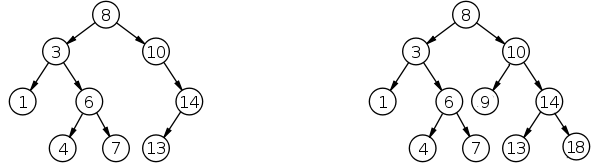
\includegraphics[width=0.80\textwidth]{img/binary-tree.png}
\end{figure}

\begin{conseil}
    La fonction \lstinline{insert(value, node)} permet d'inséret un élément dans un arbre. Exemple: \lstinline{tree.insert(9,root)}\\\\
    Télécharger le fichier ressource de la question 14 est écrivez votre code à partir de la ligne 66. 
\end{conseil}

\begin{solution}
    \textbf{Python} \\

    \lstinputlisting{solutions/question14.py} 
\end{solution}

\end{Exercice}

\section{Quiz général}

\subsection{Python}

\begin{Exercice}[2 minutes]\\
En python, 'Hello' équivaut à "Hello". 

\begin{enumerate}[label=\Alph*]
    \item - Vrai
    \item - Faux
\end{enumerate}
\begin{solution}
    \textbf{Vrai}: En python, les doubles guillemets et les guillemets sont équivalents. 
\end{solution}
\end{Exercice}


\begin{Exercice}[2 minutes]\\
Dans une fonction, nous pouvons utiliser les instructions \lstinline{print()} ou \lstinline{return}, elles ont le même rôle.
\begin{enumerate}[label=\Alph*]
    \item - Vrai
    \item - Faux
\end{enumerate}
\begin{solution}
    \textbf{Faux}\\
    \lstinline{print()} permet uniquement d'afficher un message dans la console. Autrement dit, \lstinline{print()} sert à communiquer un message à l'utilisateur final du programme, celui-ci n'ayant pas accès au code.\\\\
    \lstinline{return} est une déclaration qui s'utilise à l'intérieur d'une fonction pour renvoyer le résultat de la fonction lorsqu'elle a été appellée. Exemple: la fonction \lstinline{len(L)} renvoie la longeur de la liste~L.\\

    Admettons que nous ayons une fonction qui renvoie le double d'un nombre. Dans notre programme, nous souhaitons ajouter le résultat de cette fonction à un nombre quelconque.
    En Python, notre programme ressemblera à ça:
    \lstinputlisting{resources/question16.py}

    Notre programme renverra une erreur de type \lstinline{TypeError: unsupported operand type(s) for +: 'int' and 'NoneType'} si on remplace la ligne 2 par \lstinline{print(nombre**2)} car la fonction \lstinline{double_nombre} renverra \lstinline{None}.
\end{solution}
\end{Exercice}


\begin{Exercice}[2 minutes]\\
Lorsqu'on fait appel à une fonction, les arguments doivent nécessairement avoir le(s) même(s) noms tel(s) que définit dans la fonction. Exemple:\\
\begin{lstlisting}
def recherche_lineaire(Liste, x):
    for i in Liste:
        if i == x:
            return x in Liste
    return -1

Liste = [1,3,5,7,9]
x = 3

recherche_lineaire(Liste,x)

\end{lstlisting}
\begin{enumerate}[label=\Alph*]
    \item - Vrai
    \item - Faux
\end{enumerate}
\begin{solution}
    \textbf{Faux}\\
    Le nom des variables données en argument n'a aucune importance tant que le type de variable est respecté. Dans notre exemple, la fonction s'attend à recevoir  une \textbf{liste} comme premier argument et un \textbf{entier} comme deuxième argument. Ici, nous aurions pu nommer la liste \lstinline{nbr_impair} et x \lstinline{valeur} et ainsi appelé la fonction \lstinline{recherche_lineaire(nbr_impair, valeur)}

\end{solution}
\end{Exercice}

\begin{Exercice}[2 minutes]\\
Si le programme Python contient une erreur, celle-ci sera detectée avant l'exécution du programme. 

\begin{enumerate}[label=\Alph*]
    \item - Vrai
    \item - Faux
\end{enumerate}
\begin{solution}
    \textbf{Faux}: En Python, les erreurs sont détectées pendant l'exécution du programme.
\end{solution}
\end{Exercice}


\begin{Exercice}[2 minutes]\\
Il est possible de faire appel à une fonction définie ``plus bas'' dans le code sans que cela ne pose problème.

\begin{lstlisting}
import math

nombre_decimal_pi(4)

def nombre_decimal_pi(int):
    return round(math.pi,int)
\end{lstlisting}

\begin{enumerate}[label=\Alph*]
    \item - Vrai
    \item - Faux
\end{enumerate}
\begin{solution}
    \textbf{Faux}: À l'exception des fonctions intégrées (il s'agit des fonctions déjà intégrées au langage Python telles que \lstinline{print(), len(), abs(), etc}...). Dans les langages suivant une logique de programmation impérative (c'est le cas de Java et Python), une fonction doit nécessairement être définie \textbf{avant} d'être appelée.
    \url{https://fr.wikipedia.org/wiki/Programmation\_imp\%C3\%A9rative}
\end{solution}
\end{Exercice}


\begin{Exercice}[5 minutes]\\
Les trois fonctions suivantes renvoient-elles systématiquement des résultats identiques ?\\Les fonctions sont censées retourner le nombre \lstinline{pi} avec le nombre de décimales (au moins une et au maximum 15) indiqué en paramètre.
\begin{multicols}{3}
\begin{lstlisting}
import math

def nombre_decimal_pi(int):
    if int > 15:
        int = 15
    elif int < 0:
        int = 1
    resultat = round(math.pi,int) 
    return resultat

print(nombre_decimal_pi(-2))
print(nombre_decimal_pi(4))
print(nombre_decimal_pi(20))



\end{lstlisting}
\columnbreak

\begin{lstlisting}
import math

def nombre_decimal_pi(int):
    if int > 15:
        resultat = round(math.pi,15)
    elif int < 0:
        resultat = round(math.pi,1)
    else: 
        resultat = round(math.pi,int)
    return resultat

print(nombre_decimal_pi(-2))
print(nombre_decimal_pi(4))
print(nombre_decimal_pi(20))

\end{lstlisting}
\columnbreak

\begin{lstlisting}
import math

def nombre_decimal_pi(int):
    if int > 15:
        return round(math.pi,15)
    elif int < 0:
        return round(math.pi,1)
    else: 
        return round(math.pi,int)
    

print(nombre_decimal_pi(-2))
print(nombre_decimal_pi(4))
print(nombre_decimal_pi(20))

\end{lstlisting}
\end{multicols}

\begin{enumerate}[label=\Alph*]
    \item - Vrai
    \item - Faux
\end{enumerate}
\begin{solution}
    \textbf{Vrai}: Les trois fonctions produisent des résultats identiques. Si besoin, exécutez le code dans IntelliJ.
\end{solution}
\end{Exercice}
\subsection{Java}


\begin{Exercice}[3 minutes] \\
Observez les deux programmes suivants en Java. Lequel a-t-il une bonne structure et peut être compilé sans erreur ?

\begin{multicols}{2}
\begin{lstlisting}
//Programme A
public class Main {

    public static void main(String[] args) {
        ma_function();
        autre_fonction();
    

        static void ma_function(){
            System.out.println("Voici ma fonction!");
        }
    
        static void autre_fonction(){
            System.out.println("Une autre fonction!");
        }
    }
}



\end{lstlisting}
\columnbreak

\begin{lstlisting}
//Programme B
public class Main {

    public static void main(String[] args) {
    ma_function();
    autre_fonction();
    }

    static void ma_function(){
        System.out.println("Voici ma fonction!");
    }

    static void autre_fonction(){
        System.out.println("Une autre fonction!");
    }
}
\end{lstlisting}
\columnbreak

\end{multicols}
\begin{enumerate}[label=\Alph*]
    \item (à gauche)
    \item (à droite)
\end{enumerate}
\begin{solution}
    \textbf{Le programme B}\\
    Le fichier dans son ensemble représente une classe Java, ici la classe s'appelle \textbf{Main} (Vous aurez plus d'informations sur le fonctionnement des classes lorsque nous aborderons la programmation orientée objet). À l'intérieur de cette classe se trouve la méthode \lstinline{public static void main()}, il s'agit de la porte d'entrée de notre programme, celle que l'on exécute et celle dans laquelle nous rédigeons notre code.\\
    Les autres fonctions, qui peuvent être appelées, se définissent au sein de la classe au même échelon que la fonction \lstinline{public static void main()} comme dans le programme B ci-dessus. 
\end{solution}
\end{Exercice}

\begin{Exercice}[2 minutes] Exercice 1\\
L'indentation des lignes de code en Java est aussi importante qu'en python.
\begin{enumerate}[label=\Alph*]
    \item - Vrai
    \item - Faux
\end{enumerate}
\begin{solution}
    \textbf{Faux}
    \\En Java, le compilateur ne prend pas en compte l'indentation pour interpréter le programme, il comprend la structure à l'aide des parenthèses, des accolades et encore des point-virgules qui indiquent la fin d'une instruction. Toutefois, l'indentation est un aspect important de la programmation car elle sert à bien structurer visuellement votre code.\\\\
    En Python, l'indentation définit la structure de votre code. Elle est donc indispensable pour la bonne interprétation et la bonne exécution de votre programme. 
\end{solution}
\end{Exercice}


\end{document}
